\documentclass{report}

% ----------------------------------------------------
% PACKAGE
% ----------------------------------------------------

\usepackage{graphicx}
\usepackage{amsmath}
\usepackage{amsfonts}
\usepackage{amssymb}
\usepackage{hyperref}
\usepackage[a4paper, portrait, margin=0.75in]{geometry}
\usepackage[italian]{babel}
\usepackage{enumerate}% http://ctan.org/pkg/enumerate
\usepackage{listings}% used for cli commands

\hypersetup{
    colorlinks=true,
    linkcolor=black,
    urlcolor=blue,
}

\title{Circolo velico}
\author{Ollari Dmitri}

\begin{document}
    \maketitle
    

    \tableofcontents
    \listoffigures

    \chapter{Requisiti funzionali e diagramma UML dei casi d'uso} % (fold)
    \label{cha:Requisiti funzionali e diagramma UML dei casi d'uso}
    \section{Requisiti funzionali} % (fold)
    \label{sec:Requisiti funzionali}

    \subsection{Impiegato}
    All'avvio del sistema viene impostato un'account impiegato con credenziali username$=$\textbf{admin} e password$=$\textbf{password}, questo utente iniziale dovrà all'occorrenza creare nuovi impiegati.

    Ogni impiegato può effettuare le seguenti azioni:
    \subsubsection{Azioni sui membri}
    \begin{itemize}
      \item Modifica account
      \item Crazione account
      \item Eliminazione account
    \end{itemize}

    \subsubsection{Azioni su imbarcazioni}
    \begin{itemize}
      \item Aggiunta imbarcazione
      \item Eliminazione imbarcazione
    \end{itemize}

    \subsubsection{Azioni sulle gare}
    \begin{itemize}
      \item Aggiunta gare
      \item Eliminazione gare
    \end{itemize}
    \subsection{Membro}
    Al primo avvio il sistema risulta privo di account dedicati ai membri, dopo che un account impiegato ha creato l'account membro, quest'ultimo può compiere le seguenti operazioni:
  \begin{itemize}
    \item Controllare lo stato del proprio abbonamento annuale
    \item Se l'abbonamento annuale dovesse essere in scadenza, il sistema permette di effettuare un rinnovo
    \item Aggiunta di imbarcazioni
    \item Controllo lo stato della tassa di rimessaggio e se in scadenza, il sitema permette di effettuare il rinnovo
    \item Iscrizione alle gare disponibili
    \item Visione dello storico delle gare alle quali si è partecipati
  \end{itemize}
    


    
    % section section name (end)

    \pagebreak
    \section{Diagrammi UML dei casi d'uso} % (fold)
    \label{sec:Diagrammi UML dei casi d'uso}
    \begin{figure}[h!]
      \begin{center}
        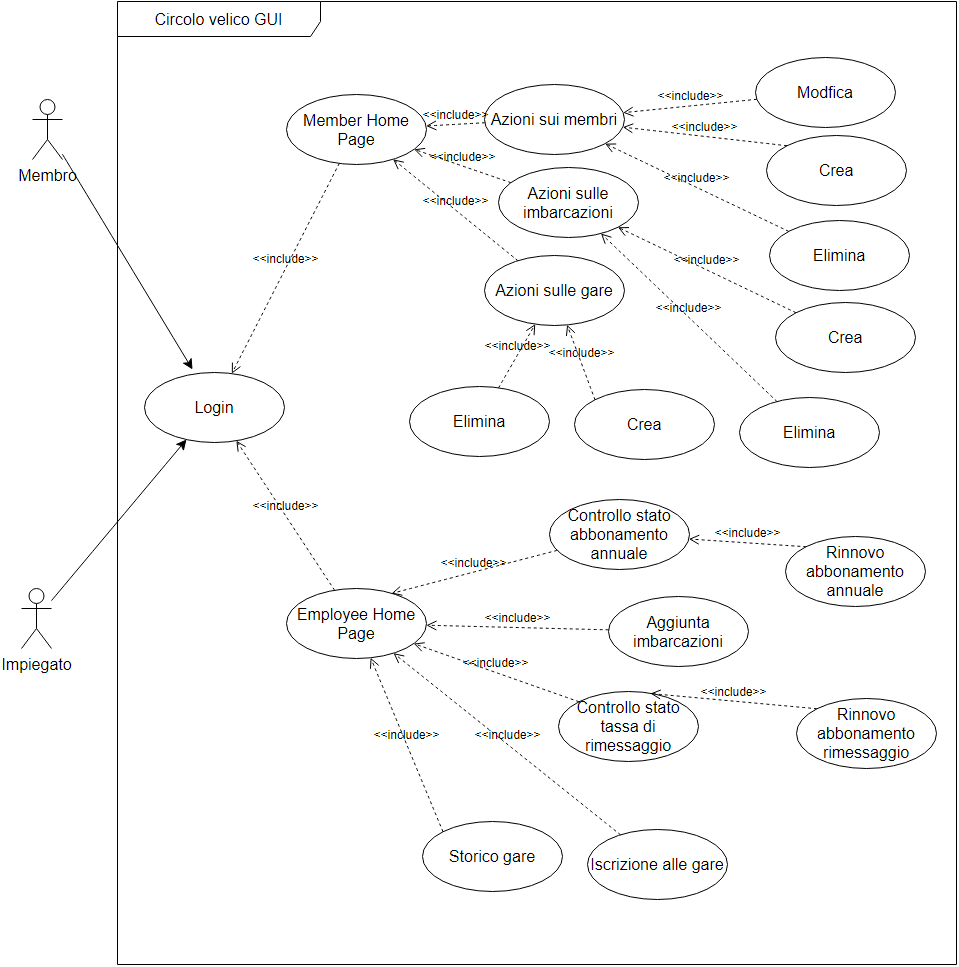
\includegraphics[width=0.95\textwidth]{./images/uml_casi_uso.png}
      \end{center}
      \caption{Diagramma UML dei casi d'uso}
      \label{fig:uml_casi_uso}
    \end{figure}
    
    
    % section section name (end)
    
    % chapter chapter name (end)


    \chapter{Diagramma UML delle classi} % (fold)
    \label{cha:Diagramma UML delle classi}

    \begin{figure}[h!]
      \begin{center}
        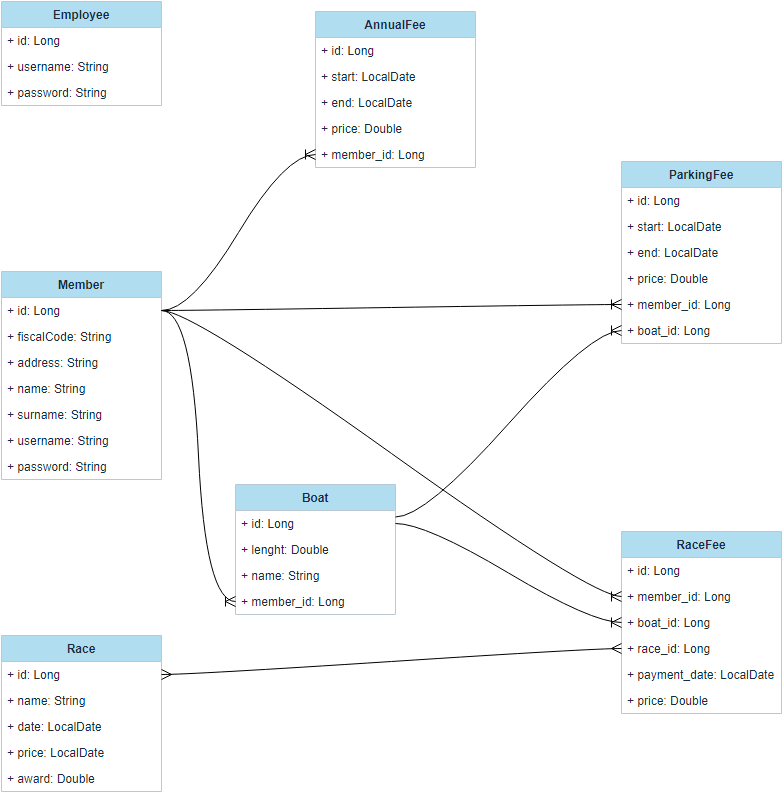
\includegraphics[width=0.80\textwidth]{./images/uml_classi.png}
      \end{center}
      \caption{Diagrammi UML delle classi}
      \label{fig:class_uml_figure}
    \end{figure}
      
    % chapter chapter name (end)


    \chapter{Descrizione di casi d'uso} % (fold)
    \label{cha:Descrizione di casi d'uso}
    \section{Rinnovo quote associative annuali}
    L'utente possiede un'abbonamento in procinto di scadenza.
    \begin{enumerate}
      \item Effettuare il login con le proprie credenziali di membro del club
      \item Nella home page comparirà in rosso una voce indicante l'imminente scadenza dell'abbonamento annuale
      \item L'utente deve recarsi nella sezione "\textbf{Tasse annuali}"
      \item Dato che l'abbonamento necessita di un rinnovo, sarà presente nella parte inferiore il pulsante adibito al rinnovo
      \item Il pulsante adibito al rinnovo del'abbonamento annuale scomparirà una volta che l'abbonamento risulta in regola
    \end{enumerate}
    \section{Aggiunta imbarcazione}
    \begin{enumerate}
      \item L'utente deve eseguire il login con le proprie credenziali
      \item L'utente deve premere il pulsante "\textbf{Barche}" per entrare nella sezione di gestione delle imbarcazioni
      \item L'utente deve compilare le specifiche del'imbarcazione da aggiungere(situate nella parte sinistra della finestra)
      \item L'utente deve confermare l'inserimento dell'imbarcazione nel sistema mediante il pulsante "\textbf{Aggiungi}"
      \item L'imbarcazione è stata aggiunta con successo
    \end{enumerate}

    \section{Iscrizione ad una gara}
    \begin{enumerate}
      \item L'utente deve eseguire il login con le proprie credenziali
      \item L'utente deve premere il pulsante "\textbf{gare}" per entrare nella sezione di gestione delle gare
      \item L'utente deve selezionare la gara alal quale desidera iscriversi
      \item L'utente deve selezionare la barca da iscrivere dal menu a tendina(in basso a sinistra)
      \item L'utente deve confermare l'iscrizione premendo il pulsante "\textbf{iscrivi barca}"
    \end{enumerate}
    
    % chapter chapter name (end)


    \chapter{Manuale} % (fold)
    \label{cha:Manuale}

    \section{Avvio applicazione}
    L'applicazione si divide in due parti principali:
  \begin{itemize}
    \item Database
    \item Backend
    \item Frontend
  \end{itemize}

  La parte di backend è responsabile della comunicazione fra il database e il frontend realizzato mediante JavaFX. 

  \subsection{Avvio di singole applicazioni}
  Trovandosi alla radice della cartella che contiene database, backend e frontend, si procede come segue:
  \subsubsection{Avvio del database}

  \begin{lstlisting}[language=bash]
  $ docker-compose -f db/docker-compose.yml up
  \end{lstlisting}    

  \subsubsection{Avvio del backend}

  \begin{lstlisting}[language=bash]
  $ java -jar backend/target/backend-0.0.1.jar
  \end{lstlisting}  

  \subsubsection{Avvio del frontend}

  \begin{lstlisting}[language=bash]
  $ java -jar frontend/target/CV-gui-0.0.1.jar
  \end{lstlisting}  


  L'applicazione si può dividere in una parte avviabile su un unico server e una parte avviabile da ogni client.

  Sul server principale si dovrà aviare il database e il backend, mentre su ogni client adibito all'accesso degli utenti e degli impiegati si dovrà avviare il frontend.
    % chapter Manuale (end)

\end{document}

